\documentclass[]{report}
\usepackage{graphicx}
\usepackage{amsmath}
\usepackage{framed}
\usepackage{subfiles}
%opening
\title{}
\author{}

\voffset=-1.5cm
\oddsidemargin=0.0cm
\textwidth = 470pt
\begin{document}

\large
\tableofcontents
\newpage
\chapter{Statistical Process Control}


%Some key tools are used in SPC. These include control charts; a focus on continuous improvement; and the design of experiments.

\section{Introduction to Statistical Process Control}
\begin{itemize}
	\item Statistical process control (SPC) is a method of quality control which uses statistical methods. 
	\item The term Statistical Process Control (SPC) is typically used in context of manufacturing processes (although it may also pertain to services and other activities), and it denotes statistical methods used to monitor and improve the quality of the respective operations. 
	\item  SPC can be applied to any process where the "conforming product" (product meeting specifications) output can be measured. 
	\item SPC is applied in order to monitor and control a process. Monitoring and controlling the process ensures that it operates at its full potential. At its full potential, the process can make as much conforming product as possible with a minimum (if not an elimination) of waste (rework or trash). 
	
	\item By gathering information about the various stages of the process and performing statistical analysis on that information, the SPC engineer is able to take necessary action (often preventive) to ensure that the overall process stays in-control and to allow the product to meet all desired specifications.
	
	\item SPC involves monitoring processes, identifying problem areas, recommending methods to reduce variation and verifying that they work, optimizing the process, assessing the reliability of parts, and other analytic operations. 
	
	\item SPC uses such basic statistical quality control methods as \textbf{quality control charts} (Shewart, Pareto, and others), capability analysis, gage repeatability/reproducibility analysis, and reliability analysis.
\end{itemize}
\section{7 Basic Tools of Quality }
{\large
	These are 7 QC tools also known as Ishikawas \textbf{7QC} tools
	\begin{description}
		\item[Cause-and-effect diagram]: Identifies many possible causes for an effect or problem and sorts ideas into useful categories.
		(also called \textit{Ishikawa} or\textit{ fishbone chart})
		
		\item[Check sheet]: A structured, prepared form for collecting and analyzing data; a generic tool that can be adapted for a wide variety of purposes.
		
		\item[Control charts]: Graphs used to study how a process changes over time.
		
		\item[Histogram]: The most commonly used graph for showing frequency distributions, or how often each different value in a set of data occurs.
		
		\item[Pareto chart]: Shows on a bar graph which factors are more significant.
		
		\item[Scatter diagram]: Graphs pairs of numerical data, one variable on each axis, to look for a relationship.
		
		\item[Stratification]: A technique that separates data gathered from a variety of sources so that patterns can be seen (some lists replace “stratification” with “flowchart” or “run chart”).
	\end{description}
	For the sake of brevity, we will only look at a couple of these.
}

%------------------------------------------------------ %
\newpage
\section{Background to  Statistical Process Control}
{
	\large
	\begin{itemize}
		\item The concepts of Statistical Process Control (SPC) were initially developed by Dr. Walter Shewhart of Bell Laboratories in the 1920's, and were expanded upon by Dr. W. Edwards Deming, who introduced SPC to Japanese industry after WWII.
		\item After early successful adoption by Japanese firms, Statistical Process Control has now been incorporated by organizations around the world as a primary tool to improve product quality by reducing process variation.
		\item Dr. Shewhart identified two sources of process variation: 
		\begin{description}
			\item[Chance variation] that is inherent in process, and stable over time, 
			\item[Assignable variation], or Uncontrolled variation, which is unstable over time - the result of specific events outside the system.
		\end{description}
		
		\item Dr. Deming relabeled chance variation as \textbf{Common Cause} variation, and assignable variation as \textbf{Special Cause} variation.
		\item Based on experience with many types of process data, and supported by the laws of statistics and probability, Dr. Shewhart devised control charts used to plot data over time and identify both Common Cause variation and Special Cause variation.
	\end{itemize}
}
%------------------------------------------------------ % 
%\newpage
%\subsection{Deming's Seminars in Japan}
%
%This article attempts to clarify the role played by W. Edwards Deming at the beginning of the modern Japanese quality control movement by summarizing and analyzing the actual content of the series of quality control lectures he gave in Japan during the summer of 1950. The primary source documents are the published lecture transcripts that Deming considered authentic.Analysis of the transcripts shows that Deming spent most of the eight-day lecture series discussing statistical process control. 
%
%
%However, he opened the lectures with extended remarks that contain a core of the philosophy for which he later became famous. Yet, significant elements of what is now known as the Deming method or Deming philosophy did not appear in the lecture series. Deming included in the lectures an extended discussion of sampling inspection that revealed his ambivalence to the subject. The transcripts show that Deming introduced to the Japanese a product design cycle of Shewhart that is distinct from the management process that the Japanese later came to call the plan-do-check-act cycle.
%------------------------------------------------------ % 

%
%
%\section{Statistical Quality Control}
%There is little difference between Statistical Quality Control (SQC) and Statistical Process Control (SPC).  At one time, there might have been some philosophical separation, but today, they exist as general synonyms.  Some prefer SQC because the idea of “quality” is larger and more encompassing than that of “process.”  Others counter this by pointing out that the term “process” is problematic by nature, whereas a focus on “quality” is symptomatic in character.  Still others looked at SQC as the management version of SPC.  The bottom line s simple – both approaches get the job done.
%
%As a notable extension of this discussion, we should acknowledge that some quality professionals are still trying to argue that Six Sigma Quality (SSQ) is just another parallax of Total Quality Management (TQM).  To better understand the true parallaxes of Six Sigma, let us consider its three primary domains.  In this manner, we can better understand how the ideas of SQC and SPC support the aims of SSQ.




\section{Contemporary Context of SPC}

\subsection{10 R packages I wish I knew about earlier}
\begin{itemize}
	\item \textit{Following material written by Drew Conway, and was published on the Yhat blog Feb 2013} \item \textit{http://blog.yhathq.com/posts/10-R-packages-I-wish-I-knew-about-earlier.html}
\end{itemize}

{\large
	\begin{itemize}
		\item \textbf{qcc} is a library for statistical quality control. Back in the 1950s, the now defunct Western Electric Company was looking for a better way to detect problems with telephone and eletrical lines.
		
		\subitem \textit{\textbf{Remark}: We will discuss these rules shortly}
		
		\item They came up with a set of rules to help them identify problematic lines. The rules look at the historical mean of a series of datapoints and based on the standard deviation, the rules help judge whether a new set of points is experiencing a mean shift.
		
%		\item The classic example is monitoring a machine that produces lug nuts. \\ Let's say the machine is supposed to produce 2.5 inch long lug nuts. We measure a series of lug nuts: 2.48, 2.47, 2.51, 2.52, 2.54, 2.42, 2.52, 2.58, 2.51. \item  Is the machine broken? Well it's hard to tell, but the \textit{Western Electric} Rules can help.
		
		\item While you might not be monitoring telephone lines, qcc can help you monitor transaction volumes, visitors or logins on your website, database operations, and lots of other processes.
	\end{itemize}}

	\subsubsection{Other Remarks}
	{\large
		\begin{itemize}
			\item Quality Control and quality assurance are important functions in most businesses from manufacturing to software development. 
			\item For most, this means that one or more people are meticulously inspecting what's coming out of the factory, looking for imperfections and validating that requirements for products and services produced are satisfied. \item Often times QC and QA are performed manually by a select few specialists, and determining suitable quality can be extremely complex and error-prone.
		\end{itemize}
\section{Some Remarks on Multivariate Techniques}
%MSQC book
{
	\large
	
	\begin{itemize}
		\item Nowadays, the intensive use of an automatic data acquisition systems and the use of
		on-line computers for process monitoring have led to an increased occurrence of
		industrial processes with two or more correlated quality characteristics, in which
		the statistical process control and the capability analysis should be performed using
		multivariate methodologies. \textit{(Edgar Santos-Fernandez)}
	\end{itemize}
}
\section{Causes of Variation}
\begin{itemize}
	\item The purpose is to control the quality of product or service outputs from a process by
	maintaining control of the process.
	\item When a process is described as being ``in control``, it means that the amount of
	variation in the output is relatively constant and within established limits that are
	deemed acceptable.
	\item There are two kinds of causes of variation in a process:
	\begin{description}
	\item[Common causes] \textit{(or chance causes)} of variation are due to factors that are
	inherent in the design of the system, and reflect the usual amount of variation
	to be expected.
	\item[Assignable causes] \textit{(or special causes)} of variation are due to unusual
	factors that are not part of the process design and not ordinarily part of the
	process.
\end{description}
	\item A \textbf{stable process} is one in which only common causes of variation affect the output
	quality. Such a process can also be described as being in a state of statistical
	control.
	\item An \textbf{unstable process} is one in which both assignable causes and common causes
	affect the output quality. (Note that, by definition, the common causes are always
	present.)
	Such a process can also be described as being out of control, particularly when the
	assignable cause is controllable.
	\item The way we set out to improve the quality of output for a process depends on the
	source of process variation.
	\item For a process that is stable, improvement can take place only by improving the
	design of the process. 
	\item \textbf{(Important)} A pervasive error in process management is \textbf{tampering},
	which is to take actions (such as making machine adjustments) that presume that a
	process is not in control, when in fact it is stable.
	\item Such actions only increase variability, and are analogous to the over-correcting that
	new drivers do in learning to steer a car. For a process that is unstable, improvement
	can be achieved by identifying and correcting assignable causes.	
\end{itemize}


\chapter{Control Charts}


\section{Control Charts}
\begin{itemize}
\item A \textbf{run chart} is a time series plot that plots levels of output quality on the vertical axis,
with respect to a sequence of time periods on the horizontal axis. In the context of
statistical process control the measurements that are graphed are typically sample
data that have been obtained by the method of rational subgroups.
\item A \textbf{control chart} is a run chart that includes the lower and upper control limits that
identify the range of variation that can be ascribed to common causes.
Any outputs that are outside of the control limits suggest the existence of assignablecause
variation.
\item The control limits are determined either by process parameters having been
specified, or by observing sample outcomes during a period of time in which the
process is deemed to be in a stable condition.
The statistical methods of process control are based on the concepts of hypothesis
testing 
\begin{figure}
\centering
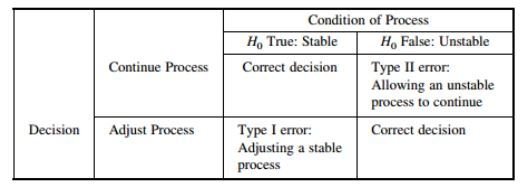
\includegraphics[width=0.7\linewidth]{images/ProcessErrors}

\end{figure}

\item The null hypothesis is that the process is stable and only common causes of
variation exist.
\item The alternative hypothesis is that the process is unstable and includes
assignable-cause variation.
\item Thus, the lower and upper control limits on a control chart are the critical values with
respect to rejecting or not rejecting the null hypothesis that the process is stable and
in control.

\item The standard practice is to place the control limits at three standard error units above
and below the hypothesized value. This \textbf{3-sigma rule} is conventionally applied for
most control chart procedures.
\item If a process is stable, not only should all sample statistics be within the control limits,
but there also should be no discernable pattern in the sequence of the sample
statistics.
\item We look at the methods for determining control limits and we describe the
interpretation of control charts for the 
\begin{enumerate}
\item process mean,
\item process range
\item process standard deviation,
\item process range, process proportion.
\end{enumerate}


\item Of these four, control charts for the mean, standard deviation, and range are designated as control charts for variables, because measurements are involved.
\item Control charts for the proportion are designated as control charts for attributes,
because counts (which are discrete rather than continuous variables) are involved.
\end{itemize}


{
	\large
	%\subsection{Control Chart}
	%\begin{itemize}
	%\item A control chart is a graphical representation of a characteristic of a process, showing plotted values of some statistic, a central line, and one or two control limits. \item It is used to determine whether a process has been operating in statistical control and is an aid to maintaining statistical control.
	%\end{itemize}
}

\subsection{Control Charts}
{\large
	\begin{itemize}
		\item The control chart is a graph used to study how a process changes over time. Data are plotted in time order. A control chart always has a central line for the average, an upper line for the upper control limit and a lower line for the lower control limit. 
		\item Units are usually the summary statistics (i.e. means or ranges) of small samples.
		\item These lines are determined from historical data. By comparing current data to these lines, you can draw conclusions about whether the process variation is consistent (in control) or is unpredictable (out of control, affected by special causes of variation).
		
		%\item Control charts for variable data are used in pairs. The top chart monitors the average, or the centering of the distribution of data from the process. The bottom chart monitors the range, or the width of the distribution. 
		%\item If your data were shots in target practice, the average is where the shots are clustering, and the range is how tightly they are clustered. Control charts for attribute data are used singly.
		
		\item (\textbf{Important}) There are several types of control chart. In the short term, we will look at the \textbf{x-bar} chart (related to mean of values from sample).
		\item (\textbf{Important}) Other types of chart include \textbf{R} charts and \textbf{S} charts (related to range and standard deviation of the values from each sample)
	\end{itemize}
}
\newpage
\subsection{Data Used for Control Chart}
\begin{figure}[h!]
\centering
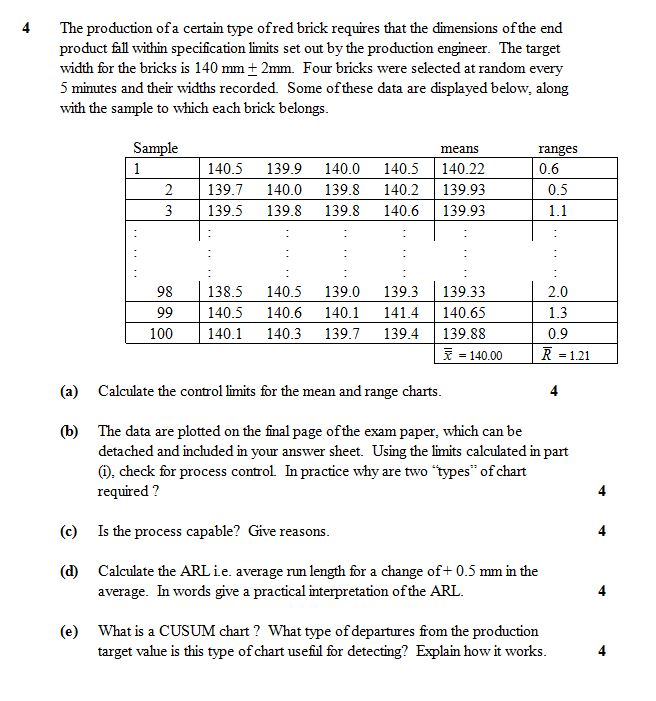
\includegraphics[width=0.8\linewidth]{images/OldExamQuestion}
\end{figure}

\newpage
\subsection{Example of a Control Chart}
This relates to a process mean.
	\begin{figure}[h!]
		\centering
		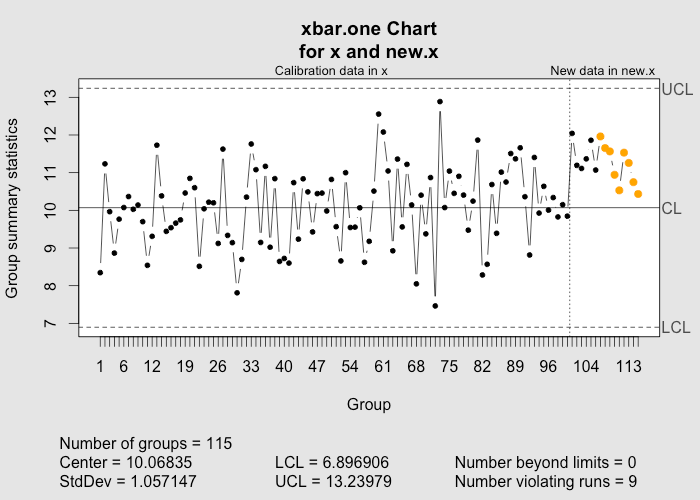
\includegraphics[width=0.9\linewidth]{./qcc-yhatexample}
	\end{figure}
\newpage
\subsection{Control Limits}
{
	\large
	\begin{itemize}
		\item Statistical tables have been developed for various types of distributions that quantify the area under the curve for a given number of standard deviations from the mean (based on the \textbf{\textit{normal distribution}} ).
		% These can be used as probability tables to calculate the odds that a given value (measurement) is part of the same group of data used to construct the histogram.
		\item Shewhart found that control limits placed at \textit{\textbf{three standard deviations from the mean}} in either direction provide an economical tradeoff between the risk of reacting to a false signal and the risk of not reacting to a true signal - regardless the shape of the underlying process distribution.
		\item If the process has a normal distribution, 99.7\% of the population is captured by the curve at three standard deviations from the mean. Stated another way, there is only a 100-99.7\%, or 0.3\% chance of finding a value beyond 3 standard deviations. Therefore, a measurement value beyond 3 standard deviations indicates that the process has either shifted or become unstable (more variability).
	\end{itemize}
}
\newpage
\begin{figure}[h!]
	\centering
	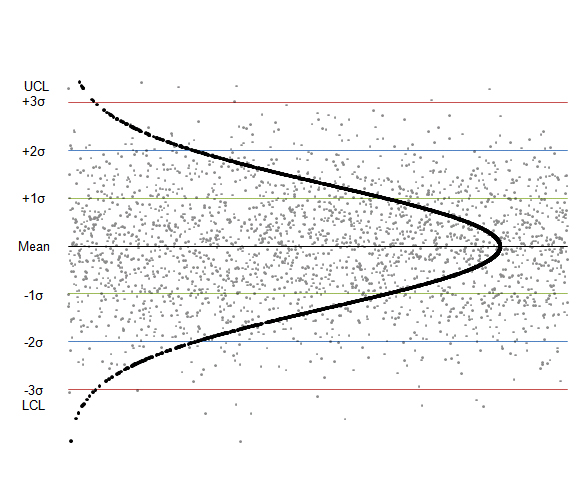
\includegraphics[width=0.8
	\linewidth]{images/ControlChart}

\end{figure}
\newpage
%===========================================================%
\section{Computing Control Limits}
\begin{framed}
Exam Paper Formulas for Control Limits
	\begin{itemize}
\item Process Mean


	
	\[ \bar{\bar{x}} \pm 3\frac{\bar{s}}{c_4\sqrt{n}}\]
\item Process Standard Deviation	
	\[ \bar{s} \pm 3\frac{c_5\bar{s}}{c_4}\]
\item Process Range	
	\[\left[ \bar{R}D_3, \bar{R}D_4\right]\]
	\end{itemize}	
	\end{framed}
\begin{figure}[h!]
\centering
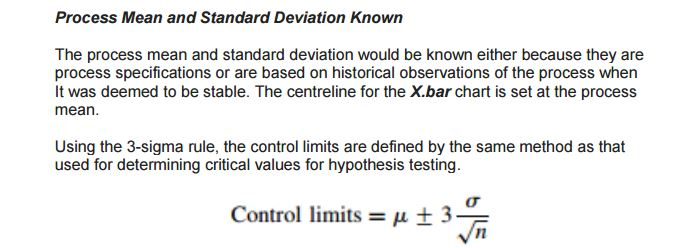
\includegraphics[width=1.0\linewidth]{images/computingControlLimits1a}

\end{figure}
\newpage
\begin{figure}[h!]
	\centering
	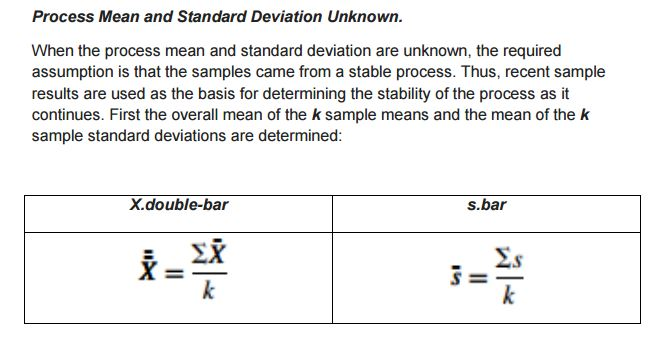
\includegraphics[width=1.0\linewidth]{images/computingControlLimits1b}
	
\end{figure}
\begin{figure}[h!]
	\centering
	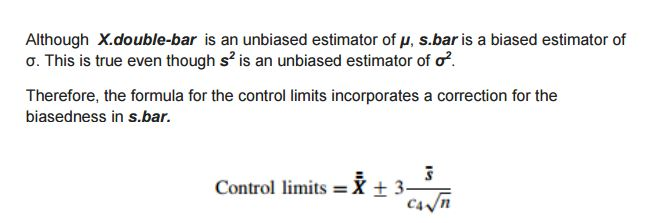
\includegraphics[width=1.0\linewidth]{images/computingControlLimits2}

\end{figure}
\newpage
%===========================================================%
\section{Control Limits: Worked Example}
\begin{figure}[h!]
\centering
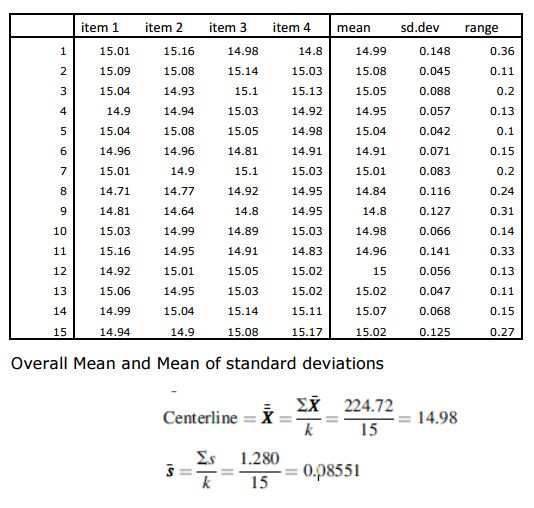
\includegraphics[width=1\linewidth]{images/WorkedExample1-data}
\end{figure}
\newpage
\begin{figure}[h!]
\centering
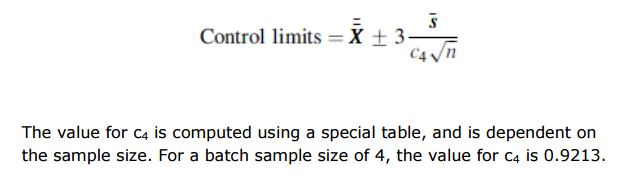
\includegraphics[width=1\linewidth]{images/WorkedExample1-formula}
\end{figure}
\begin{figure}[h!]
	\centering
	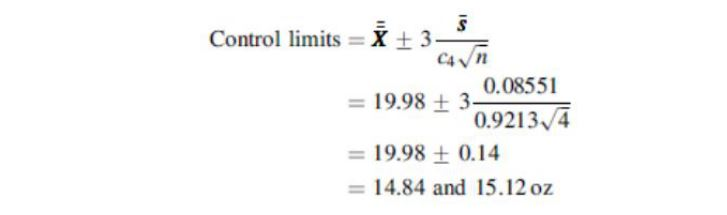
\includegraphics[width=1\linewidth]{images/WorkedExample1-solution}
\end{figure}
\newpage
\begin{figure}[h!]
\centering
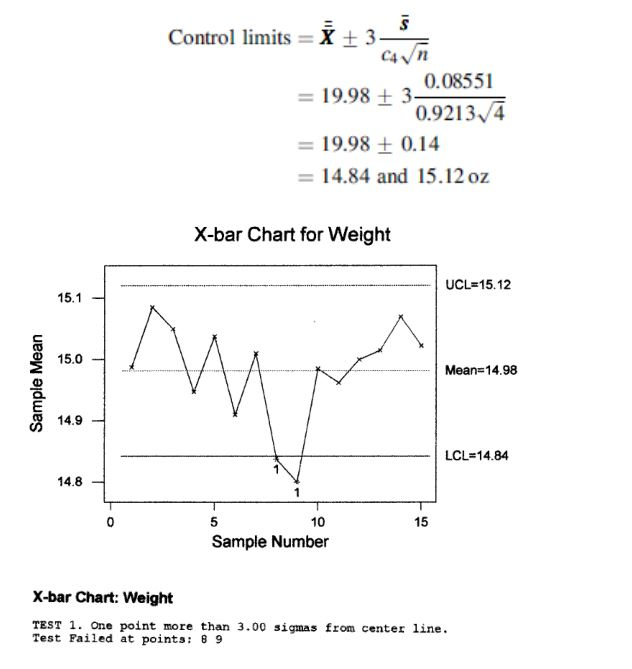
\includegraphics[width=1\linewidth]{images/WorkedExample1-chart}

\end{figure}

\newpage
%===========================================================%

\section{Nelson Rules for Interpreting Control Charts}
{\large
	\begin{itemize}
		\item The eight tests used in statistical process control were developed by Lloyd S. Nelson, a process control expert. They are
		based on his determination that the identified patterns are very unlikely to occur in stable processes.
		
		\item Thus
		the existence of any of these patterns in an $\bar{X}$ chart indicates that the process may be unstable, and that one or
		more assignable causes may exist. 
		
		\item The table on the next page contains examples of test failure for each of the eight tests,
		with a description for each graph as to what is required for the illustrated test failure.
		
		\item In practice, tests 1,2 and 7 are considered the three most useful.
	\end{itemize}
}
{
	\large
	\subsection{Descriptions of Tests}
	\begin{description}
		\item[Test 1 - 3 sigma rule] Identifies points outside of the control limits\\
		Test 1 identifies points that are more standard deviations from the center line. Test 1 is
		universally recognized as necessary for detecting out-of-control situations. It has a
		false alarm rate of only 0.27\%.
		
		\item[Test 2] Identifies shifts in the means \\
		Test 2 signals when 9 points in a row fall on the same side of the center line.  The use of Test 2
		significantly increases the sensitivity of the chart to detect small shifts in the mean.
		
		When test 1 and test 2 are used together, significantly fewer subgroups are needed
		to detect a small shift in the mean than are needed when test 1 is used alone.
		Therefore, adding test 2 helps to detect common out-of-control situations and
		increases sensitivity enough to warrant a slight increase in the false alarm rate.
	\end{description}
}
\newpage
\begin{figure}[h!]
	% 
	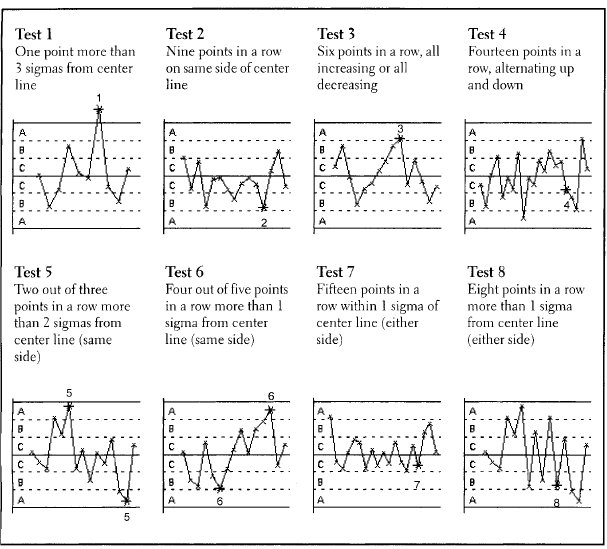
\includegraphics[scale=0.85]{images/WECOtests}\\
	%\caption{WECO Tests}\label{WECO}
\end{figure}


\newpage
{
	\large
	\begin{description}
		\item[Test 3] $k$ points in a row, all increasing or all decreasing\\
		Test 3 is designed to detect drifts in the process mean.\\
		However, when test 3 is used in addition to test 1 and test 2, it does not
		significantly increase the sensitivity of the chart to detect drifts in the process
		mean.
		
		
		\item[Test 4] $k$ points in a row, alternating up and down\\
		Although this pattern can occur in practice, it is recommended to search for any
		unusual trends or patterns rather than test for one specific pattern.
		\item[Test 5] $k$ out of k=1 points $> 2$ standard deviations from center line\\
		This test is not quite as informative because it did not
		uniquely identify special cause situations that are common in practice.
		\item[Test 6] $k$ out of k+1 points $> 1$ standard deviation from the center line\\
		This test is not quite as informative because it did not
		uniquely identify special cause situations that are common in practice.
		
		\item[Test 7] Identifies control limits that are too wide\\
		Test 7 signals when 12 or 15 points in a row fall within 1 standard deviation of the
		center line.\\ Test 7 is used only for the $\bar{X}$ chart when the control limits are
		estimated from the data. When this test fails, the cause is usually a systemic source
		of variation (stratification) within a subgroup, which is often the result of not 
		forming rational subgroups. 
		\item[Test 8] $k$ points in a row $> 1$ standard deviation from center line (either
		side)\\
		This test is not quite as informative because it did not
		uniquely identify special cause situations that are common in practice.
	\end{description}
}
\newpage
\subsection{Interpreting Control Charts}
\begin{itemize}
\item The most obvious test in terms of its rationale is Test 1, which simply requires that at
least one value of \textbf{X.bar} be beyond Zone A. For a sample mean to be beyond three
standard errors from the centre-line is of course very unlikely in a stable process.
\item The other seven patterns also are very unlikely.
The one test whose rationale is not obvious is Test 7, which requires that 15
consecutive values of \textbf{X.bar} be in Zone C, which is within one standard error of the
centre-line.
\item Although this kind of pattern would seem to be very desirable, it is also very unlikely.
It may, for example, indicate that the process standard deviation was overstated in
the process specifications or that the sample measurements are in error. Whatever
the cause, the results are too good to be true and therefore require investigation.
\end{itemize}



\section{Multivariate Normal}
{\large
	\begin{itemize}
		\item The multivariate normal distribution or multivariate Gaussian distribution, is a generalization of the one-dimensional (univariate) normal distribution to higher dimensions.\item One possible definition is that a random vector is said to be k-variate normally distributed if every linear combination of its k components has a univariate normal distribution. 
		%\item However, its importance derives mainly from the multivariate central limit theorem.
		\item The multivariate normal distribution is often used to describe, at least approximately, any set of (possibly) correlated real-valued random variables each of which clusters around a mean value.
	\end{itemize}
}
\begin{figure}[h!]
	\centering
	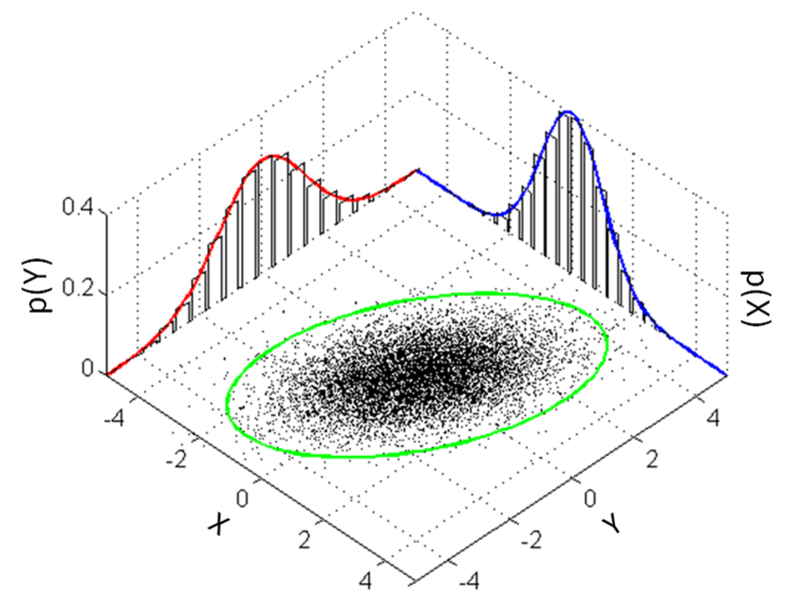
\includegraphics[width=0.7\linewidth]{./793px-MultivariateNormal}
	\caption{}
	\label{fig:793px-MultivariateNormal}
\end{figure}
%------------------------------------------------------ % 
\newpage
\subsection{Testing for Normality}
%MSQC
{
	\large
	\textbf{Graphical Methods}
	\begin{itemize}
		\item Histograms
		\item Normal Probability Plots
	\end{itemize}
	
	\noindent\textbf{Hypothesis Tests for Univariate Data}
	\begin{itemize}
		\item Shapiro-Wilk Test (inbuilt with \texttt{R})
		\item D'Agostino Test (MSQC package)
	\end{itemize}
	\bigskip
	
	\noindent\textbf{Hypothesis Tests for Multivariate Data}
	\begin{itemize}
		\item Mardia Test (MSQC package)
		\item Henze and Zirkler (MSQC package)
		\item Royston Test (MSQC package)
	\end{itemize}
	
	
}
\newpage
\subsubsection{The bimetal data set (MSQC package)}
{\large
	\begin{itemize}
		\item Bimetal thermostat has innumerable practical uses. These types of thermostats hold
		a bimetallic strip composed by two strips of different metals that convert the
		changing of temperature in mechanical displacement due to the difference in
		thermal expansion.
		\item Certain type of strip composed of brass and steel is analyzed in a quality
		laboratory by testing the deflection, curvature, resistivity, and hardness in low
		and high expansion sides.
	\end{itemize}
	\begin{framed}
		\begin{verbatim}
		> tail(bimetal1)
		deflection curvature resistivity Hardness low side Hardness high side
		[23,]      20.76     39.98       14.98             22.29             26.03
		[24,]      21.00     40.11       15.17             22.04             25.99
		[25,]      20.57     39.73       14.35             22.02             25.80
		[26,]      20.78     39.83       15.27             21.60             25.89
		[27,]      20.96     40.03       15.26             21.98             25.94
		[28,]      21.14     39.93       14.98             21.84             25.98
		
		\end{verbatim}
	\end{framed}
}
\newpage
\begin{figure}[h!]
	\centering
	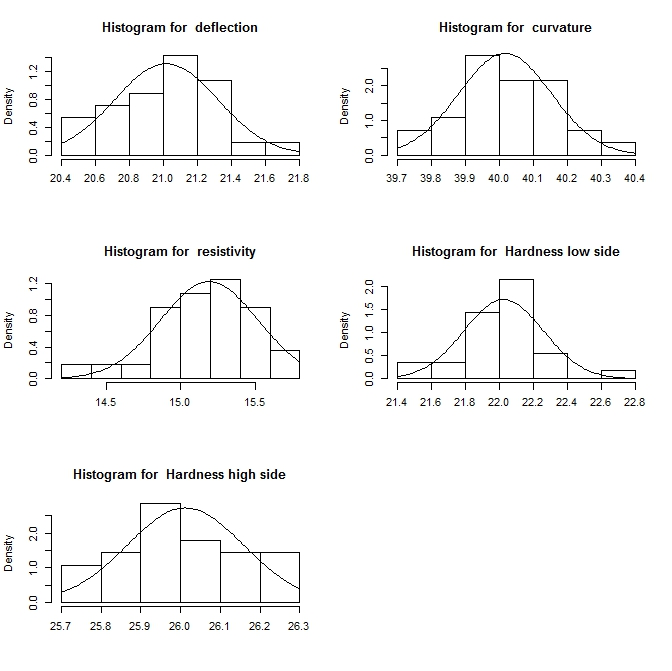
\includegraphics[width=0.9\linewidth]{images/MSQC-bimetal1hist}
	\caption{}
	\label{fig:MSQC-bimetal1hist}
\end{figure}
\newpage
\begin{figure}[h!]
	\centering
	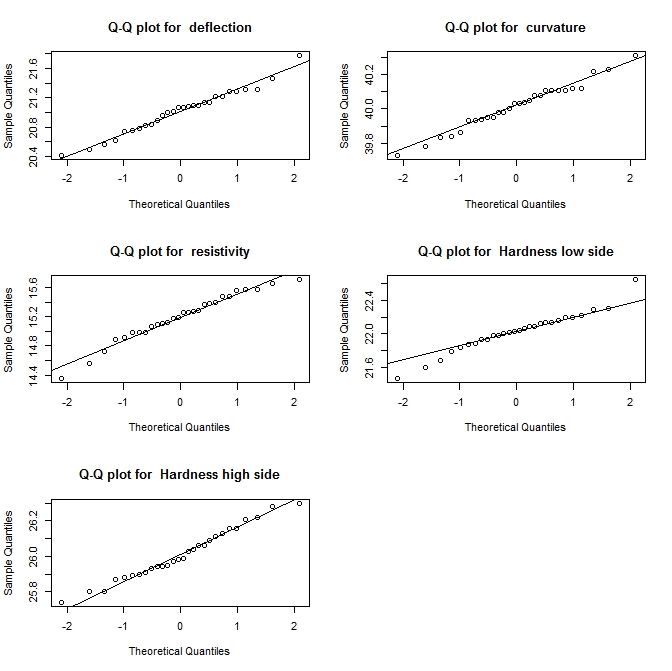
\includegraphics[width=0.9\linewidth]{images/MSQC-bimetal1qq}
	\caption{}
	\label{fig:MSQC-bimetal1qq}
\end{figure}
\newpage
\subsubsection{D'Agostino Test (MSQC Pacakge)}
\begin{itemize}
	\item Using the bimetal1 data set in MSQC package
\end{itemize}
\begin{framed}
	\begin{verbatim}
	> for (i in 1 : 5){
	+  DAGOSTINO(bimetal1[,i])
	+  }
	D'Agostino Test
	Skewness
	Skewness coefficient: 0.0831225 
	Statistics: 0.2117358 
	p-value: 0.8323131 
	Kurtosis
	The kurtosis coefficient: 3.0422 
	Statistics: 0.591983 
	p-value: 0.553862 
	Omnibus Test
	Chi-squared: 0.3952759 
	Degree of freedom: 2
	p-value: 0.8206669 
	....
	....
	D'Agostino Test
	Skewness
	Skewness coefficient: -0.04173762 
	Statistics: -0.1063873 
	p-value: 0.9152751 
	Kurtosis
	The kurtosis coefficient: 4.162062 
	Statistics: 1.675258 
	p-value: 0.09388364 
	Omnibus Test
	Chi-squared: 2.817807 
	Degree of freedom: 2
	p-value: 0.2444111 
	\end{verbatim}
\end{framed}
\newpage
\subsubsection{Some Multivariate (MSQC Package)}
\begin{framed}
	\begin{verbatim}
	> MardiaTest(bimetal1)
	$skewness
	[1] 6.982112
	
	$p.value
	[1] 0.585327
	
	$kurtosis
	[1] 33.77373
	
	$p.value
	[1] 0.3490892
	
	> 
	>
	>
	> HZ.test(bimetal1)
	[1] 0.6068650 0.7709586
	> 
	> 
	> Royston.test(bimetal1)
	test.statistic        p.value 
	1.1814742      0.9364221 
	\end{verbatim}
\end{framed}

\end{document}


\subsubsection{Box Cox Transformation}
\begin{itemize}
	\item The Box-Cox transforms nonnormally distributed data to a set of  data that has approximately normal distribution. 
\end{itemize}

\newpage
%------------------------------------------------------ % 





\chapter{Review Questions (Theory Questions)}

\begin{enumerate}
	\item  Differentiate common (or chance) causes of variation in the quality of process output from
	assignable (or special) causes.
	\item  Differentiate a stable process from an unstable process.
	\item Other than applying the 3-sigma rule for detecting the presence of an assignable cause, what else do we look for when studying a control chart?
	\item Describe how the output of a stable process can be improved. What actions do not improve a
	stable process, but rather, make the output more variable?
	\item  What is the purpose of maintaining control charts?
	\item What is tampering in the context of process control?
	
\end{enumerate}
\chapter{Process Capability Indices}
\subfile{ProcessCapabilityLectureNotes.tex}
\end{document}

